\documentclass[12pt,a4paper]{report}
\usepackage[utf8]{inputenc}
\usepackage[spanish]{babel}
\usepackage{amsmath}
\usepackage{amsfonts}
\usepackage{amssymb}
\usepackage{graphicx}
\usepackage[left=2cm,right=2cm,top=2cm,bottom=2cm]{geometry}
\author{Oscar Cruz Cervantes}
\title{EV_2_3_giro_de_un_motor_de_cprriente_directa}

\begin{document}
\begin{center}
Oscar Cruz Cervantes\\
18311638\\
Giro de un motor de corriente directa\\
Sistemas Electronicos de Interfaz\\

\includegraphics[scale=1.5]{01.png}\\
Ingenierìa Mecatronica\\
\end{center}
\newpage
\subsection{Puente H}

Un Puente en H es un circuito electrónico que generalmente se usa para permitir a un motor eléctrico DC girar en ambos sentidos, avance y retroceso. Son ampliamente usados en robótica y como convertidores de potencia. Los puentes H están disponibles como circuitos integrados, pero también pueden construirse a partir de componentes discretos.\\
El término "puente H" proviene de la típica representación gráfica del circuito. Un puente H se construye con 4 interruptores (mecánicos o mediante transistores). Cuando los interruptores S1 y S4 (ver primera figura) están cerrados (y S2 y S3 abiertos) se aplica una tensión positiva en el motor, haciéndolo girar en un sentido. Abriendo los interruptores S1 y S4 (y cerrando S2 y S3), el voltaje se invierte, permitiendo el giro en sentido inverso del motor.
\begin{center}
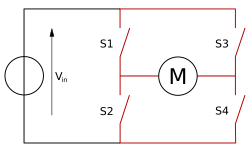
\includegraphics[scale=1.5]{02.png}
\end{center}
\subsection{Funcionamiento}
El puente de H funciona mediante el uso de 4 diodos estos se conectan al motor de manera de manera que el diodo 1 y el cuatro se conectan haciendo una rectificacion de onda completa en el ciclo positivo haciendo girar el motor y los diodos 2 y 3 se conectan al motor de manera inversa haciendo haciendo una rectificacion de onda completa en el ciclo negativo, esto provoca que el motor gire en sentido contrario.


\cite{PUENTEH}
\bibliographystyle{apalike}
\bibliography{PUENTEH}

\end{document}